\newpage
\section{Design} \label{sec:design}

\subsection{Algorithm library}

The library is designed to be modular. The code is aimed at supporting research in DRL. Most of it is written in python in a highly modular way, such that researchers can easily swap components, transform them or write new ones with little effort. Figure \ref{fig:sac-uml} is a UML class diagram for SAC. The SAC class contains the main logic of the algorithm. The actor network, critic network, and the replay buffer are spun off from the main logic to form separate classes. These three classes are then passed as arguments into the SAC class. In this way, SAC can use neural networks and replay buffers with different mechanisms, and can also share certain components with other algorithm classes.

\begin{figure}[htbp]
   \centering
   \includesvg[inkscapelatex=false,pretex=\fontsize{9}{12}\selectfont,width=\textwidth]{SAC-UML}
   \caption{UML class diagram of the Soft Actor-Critic algorithm}
   \label{fig:sac-uml}
\end{figure}

To prevent algorithm classes from working with the wrong components, this library uses Python's duck typing feature for static type checking when passing arguments. This means that when the wrong component is passed in, static analysis tools like \textit{mypy} will report an error to alert the user.

As shown in Figure \ref{fig:sac-uml}, the API of the algorithm class is designed such that the argument list only exposes hyperparameters and necessary components, while member methods only expose gradient stepping and action computation. By designing the API in this way, it forces the API to be highly consistent with the algorithm in the paper in terms of cognitive load, thereby avoiding potential usage barriers caused by the API containing unfamiliar information to the user \cite{ref:api}.

In software design, unit testing is commonly used to maintain the stability of the API and critical logic. This library also utilises unit testing, but not for maintaining API stability. This is because DRL is inherently an unstable field, with algorithms evolving rapidly. Therefore, maintaining API stability may become a hindrance in the future for continuously updating this library.

As this is an algorithm library, a relatively lower-level components in an application software, its compatibility is closely related to its usability. To achieve high compatibility, this library sacrifices the opportunity to use advanced Python features to simplify the code, keeping the minimum Python version at 3.8 to ensure compatibility with ROS Noetic. On the other hand, the library tries to minimise dependencies on other software packages to avoid conflicting with dependencies of other packages. It only use \textit{Pytorch} for tensor computation, \textit{attr} for enhancing object-oriented paradigm, and \textit{toolz} for enhancing functional programming paradigm. Other development-specific dependencies, such as debugger, profiler, and linter, are put in to a separated dependency group which only to be installed by developer manually.

The library is packaged with the latest Python packing standard, PEP 518 \cite{ref:pep518}. This ensures that the library can be easily distributed on the web and easily installed on any computer with a Python interpreter.

The development of this library is version-controlled using Git in conjunction with GitHub. The source code, development logs, and statistics can be found here: \url{https://github.com/MinghongAlexXu/deeprl}.

\subsection{Training environment}

Since the purpose is to study DRL using mapless navigation as an example, the training environment is kept as simple as possible. The training environment is modelled in the Gazebo Classic simulator, with a square enclosure measuring $3m \times 3m$ and a flat ground, as shown in Figure \ref{fig:birdview}. TurtleBot3, a simplest differential drive robot with a 2d LiDAR, is chosen as the agent. ROS Noetic is used for communication between the training program and the simulator as a message queue.

\begin{figure}[htbp]
   \centering
   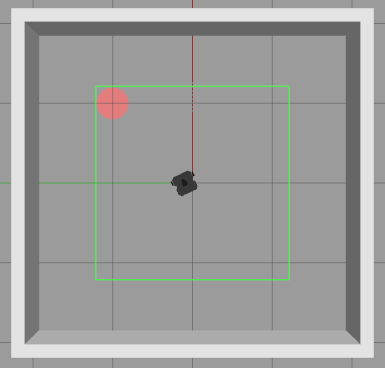
\includegraphics[width=0.6\textwidth]{images/birdview-of-env.png}
   \caption{Aerial view of the training environment in Gazebo Classic.}
   \label{fig:birdview}
\end{figure}

{
\setlength{\parindent}{0pt}
\setlength{\parskip}{1.5ex}

The environment spaces and reward signal are defined below.

Observed state space:
\begin{equation*}
    S = (\text{lidar}, \text{imu}, \text{distance}),
\end{equation*}
where \textit{lidar} is the data from LiDAR, \textit{imu} is the data from 
 the inertial measurement unit (IMU), and \textit{distance} is the relative distance of the navigation goal w.r.t the robot.

Action space:
\begin{equation*}
    A = (\text{linear}, \text{angular}),
\end{equation*}
where \textit{linear} and \textit{angular} are respectively the linear and angular velocity of the robot.

Reward shaping
\begin{equation*}
    \mathcal{r}(s_t, a_t) = \begin{cases}
    \mathcal{r}_\text{goal}, &\text{if $d_t < d_\text{th}$}\\
    \mathcal{r}_\text{obstacle}, &\text{if $x_t < x_\text{th}$}\\
    c (d_t - d_{t-1}), &\text{otherwise.}
    \end{cases}
\end{equation*}
Notice that $c$ is an amplification factor and a parameter of the environment, $s_t \in S$, and $a_t \in A$.

}

To train the obstacle avoidance ability, two training environments with obstacles were designed. In the first environment, as shown in Figure \ref{fig:cluttered}, the obstacles are relatively small, leaving a lot of space for the robot to move. In the other environment, as shown in Figure \ref{fig:escape}, the obstacles are larger, and the paths available for the robot to move are relatively more limited.

\begin{figure}[htbp]
\centering
\begin{subfigure}[b]{0.49\textwidth}
   \centering
   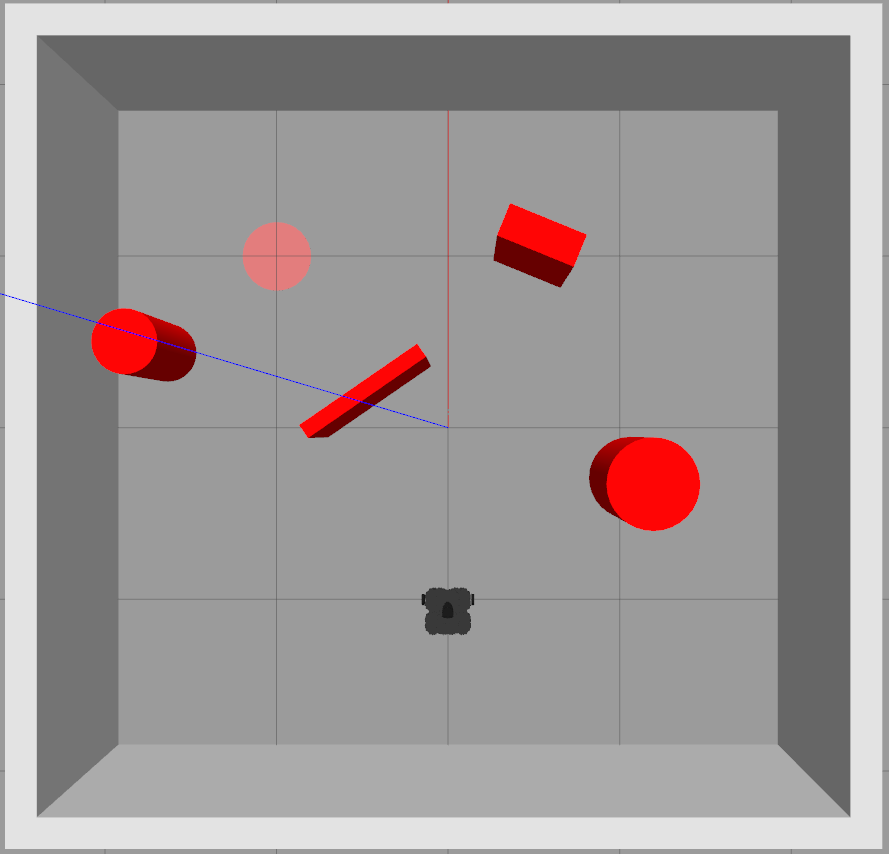
\includegraphics[width=\textwidth]{cluttered.png}
   \caption{An obstacle slightly blocks the path of moving to the goal.}
   \label{fig:cluttered}
\end{subfigure}
\begin{subfigure}[b]{0.49\textwidth}
   \centering
   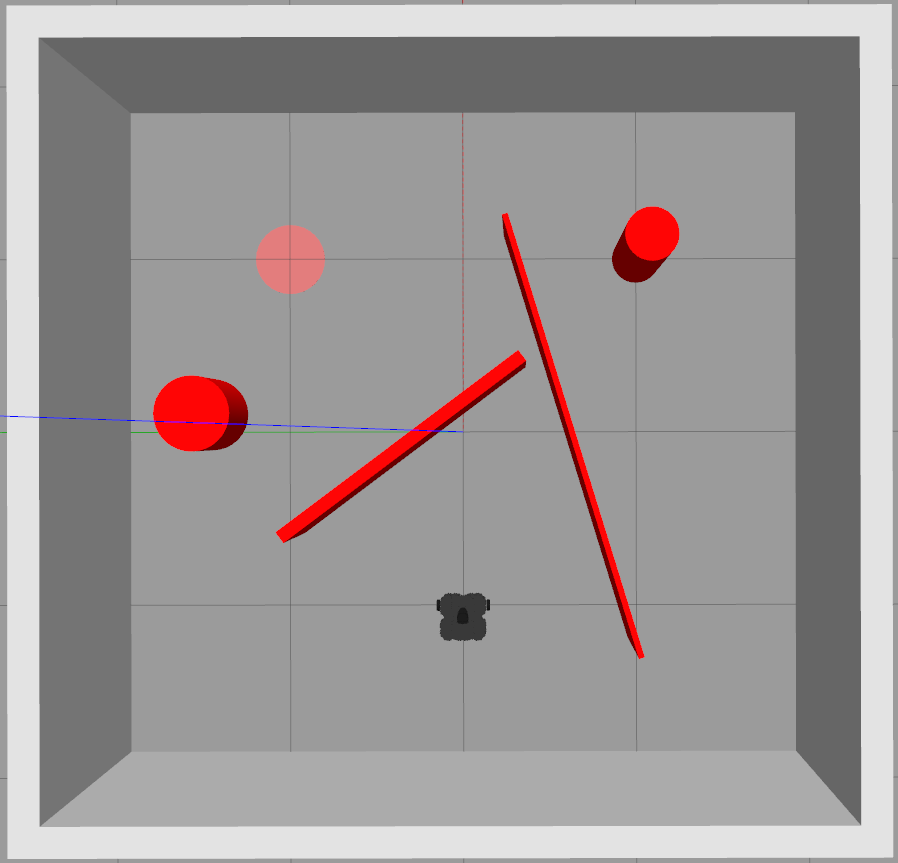
\includegraphics[width=\textwidth]{escape.png}
   \caption{Obstacles almost completely block the path of moving to the goal. The robot needs to first escape to one end of the obstacle before it can approach the goal.}
   \label{fig:escape}
\end{subfigure}
\caption{Environments with obstacles}
\end{figure}

The code for the training environments is available on \url{https://github.com/TACPSLab/SNN4RoboticControl}.
